\section{}

\textbf{Tiempo de lectura:} \{s02-reading-time\}

Ahora que sabemos que todos los sistemas operativos hacen lo mismo, pero
que el «cómo» lo hacen difiere de un tipo de sistema informático a otro,
vamos a ver los tipos de sistemas informáticos, las características de
los sistemas operativos que los gestionan y cómo han evolucionado a lo
largo de la historia.

\section{Mainframe}\label{_mainframe}

Los \textbf{ordenadores centrales} o \emph{\textbf{{}mainframes}} fueron
los primeros computadores utilizados en muchas aplicaciones comerciales
y científicas. Se caracterizan no tanto por la potencia de su CPU como
por su: gran capacidad de memoria, gran capacidad de almacenamiento
secundario, gran cantidad de dispositivos de E/S y rapidez de estos y
alta fiabilidad.

Los \emph{mainframes} pueden funcionar durante años sin problemas ni
interrupciones y las reparaciones se realizan sin detener su
funcionamiento.

La mayor diferencia entre los superordenadores y los
\emph{mainframes}\hyperref[Wikipedia-Mainframe]{???} está en que los
primeros se centran en resolver problemas limitados por la velocidad de
cálculo ---lo cual requiere miles de CPU de alto rendimiento--- mientras
que los segundos se centran en la fiabilidad y en problemas limitados
por la E/S ---por lo que los \emph{mainframes} suelen tener «solo» entre
una y varias docenas de CPU---.

Los \emph{mainframes} aparecieron a finales de la década de los 50 del
siglo pasado y han seguido evolucionando hasta la actualidad, por lo que
dentro de este tipo de sistemas nos encontramos con varias categorías.

\subsection{Sistemas de procesamiento por
lotes}\label{_sistemas_de_procesamiento_por_lotes}

{} {} Los primeros \emph{mainframes} eran enormes máquinas operadas
desde una consola y conectados a lectores de tarjetas perforadas,
dispositivos de cinta e impresoras.

Para imágenes y más información sobre las tarjetas perforadas, véase
\href{https://en.wikipedia.org/wiki/Computer_programming_in_the_punched_card_era}{«Computer
programming in the punched card era --- Wikipedia»}.

El trabajo era preparado por cada programador ---normalmente en tarjetas
perforadas--- y entregado al operador del sistema, que era quién tenía
acceso al sistema y la responsabilidad de ejecutar los programas y
devolver los resultados al programador correspondiente.

No había sistema operativo y el operador debía cargar y ejecutar cada
programa de uno en uno.

\begin{figure}
\centering
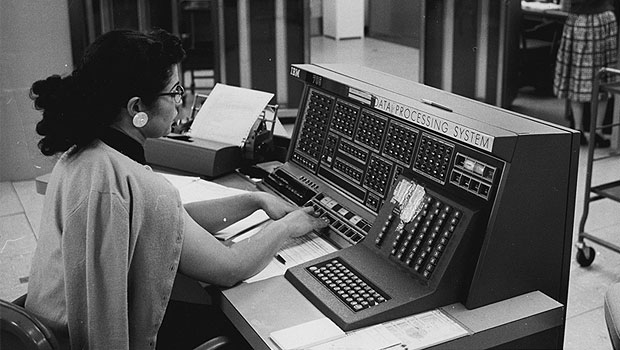
\includegraphics[keepaspectratio]{media/C02_tipos_de_sistemas/consola_ibm_705.jpg}
\caption{Operadora en la consola de un mainframe IBM 705 --- Fuente:
\href{https://www.ibm.com/history/700}{IBM}}\label{fig-consola-ibm-705}
\end{figure}

Estos sistemas se convirtieron en \textbf{sistemas de procesamiento por
lotes} o \textbf{sistemas en \emph{batch}} cuando se comenzó a utilizar
un pequeño programa ---llamado \textbf{monitor del sistema}--- cuya
función era cargar y ejecutar sin interrupción un conjunto ---o lote---
de programas.

Para preparar los lotes, por lo general, el operador cargaba previamente
en cinta magnética el conjunto de programas a partir de las tarjetas
perforadas proporcionadas por los programadores. Como se ilustra en la
\hyperref[fig-sistemas-procesamiento-lotes]{Gestión de trabajos en
sistemas de procesamiento por lotes.}, para ello se utilizaba un
ordenador autónomo ---independiente del \emph{mainframe}--- con lector
de tarjetas y unidad de cinta. Posteriomente, el operador movía la cinta
con el conjunto de programas a la unidad de cinta de entrada del
\emph{mainframe} y lanzaba la ejecución del \textbf{monitor del
sistema}, para que este se encargara de ir leyendo y ejecutando cada uno
de los programas. Para obtener mayor rendimiento, los resultados de los
programas se escribían en una unidad de cinta diferente. Cuando
terminaba la ejecución de todo el conjunto, el operador llevaba la cinta
a otro ordenador autónomo para leer los resultados e imprimrlos, con el
objeto de entregárselos a los programadaores.

\begin{figure}
\centering
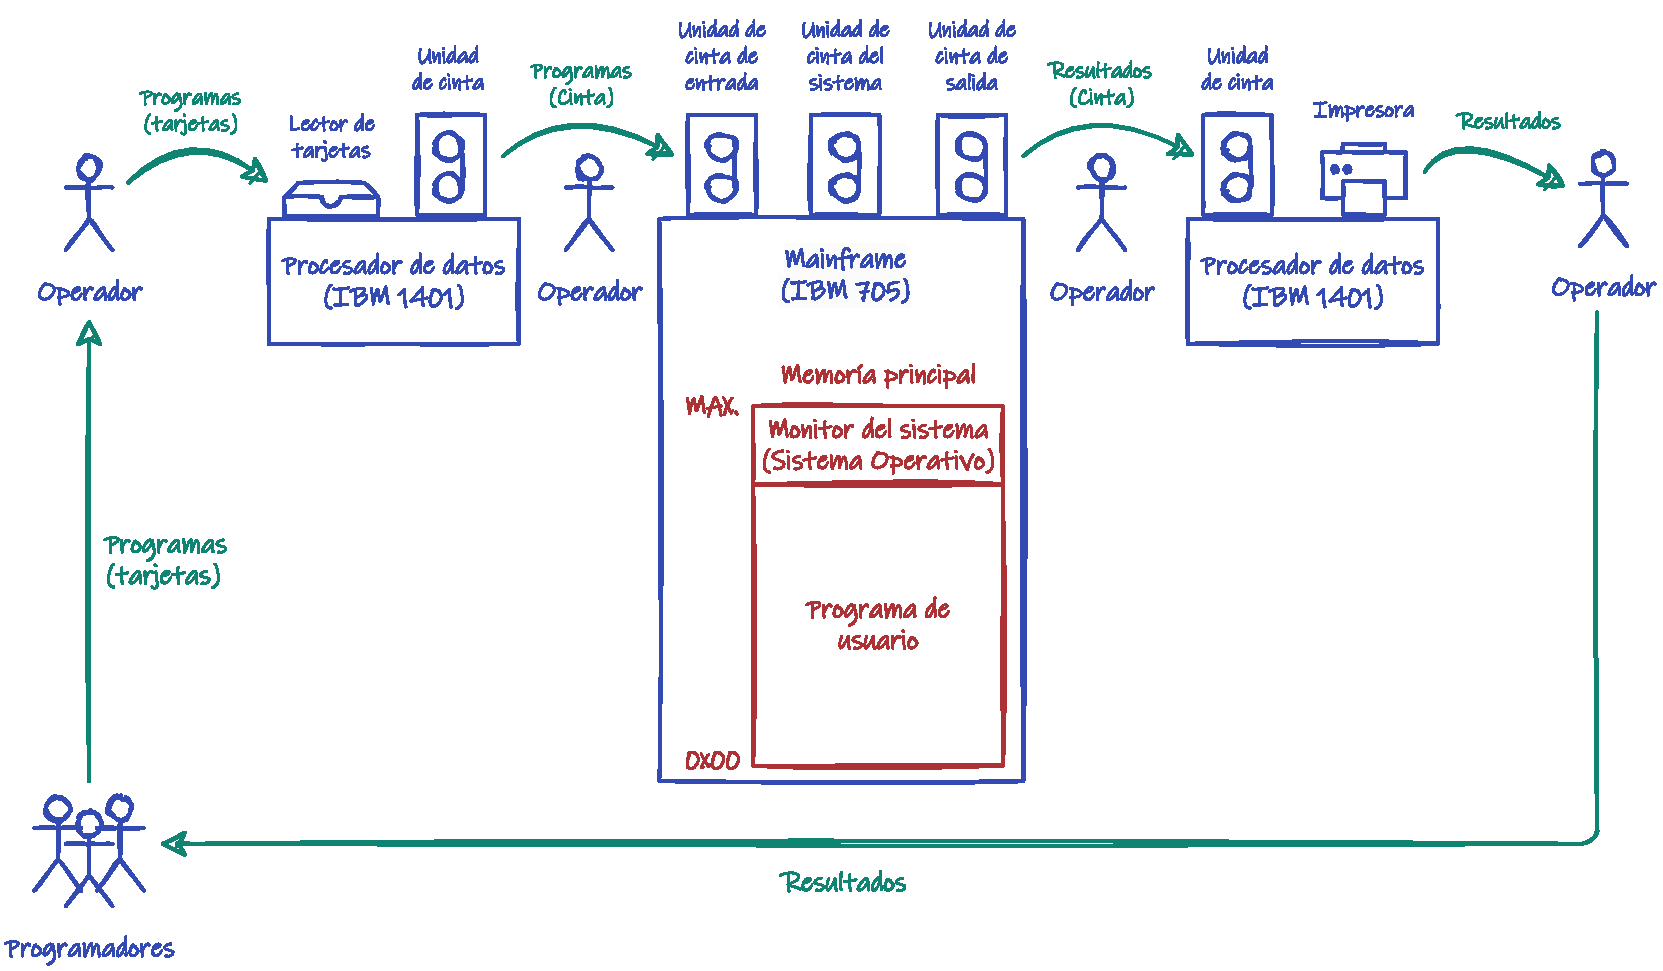
\includegraphics[width=0.8\textwidth]{media/C02_tipos_de_sistemas/sistemas_procesamiento_lotes.pdf}
\caption{Gestión de trabajos en sistemas de procesamiento por
lotes.}\label{fig-sistemas-procesamiento-lotes}
\end{figure}

El \textbf{{}monitor del sistema} es un predecesor de los sistemas
operativos y tenía las siguientes características:

\begin{itemize}
\item
  Permanecía cargado durante todo el tiempo en la memoria del sistema
  (véase la \hyperref[fig-sistemas-procesamiento-lotes]{Gestión de
  trabajos en sistemas de procesamiento por lotes.}).
\item
  Su única tarea era cargar y transferir automáticamente la ejecución de
  un programa al siguiente cuando el anterior terminaba.
\item
  El mayor inconveniente de este tipo de sistemas era que la CPU
  permanecía mucho tiempo desocupada porque era ---y sigue siendo---
  varios órdenes de magnitud más rápida que los dispositivos de E/S.
\end{itemize}

Cualquier programa necesita realizar operaciones de E/S para obtener los
datos requeridos para sus cálculos ---guardados en tarjetas perforadas y
unidades de cinta o, si hablamos de hoy en día, en discos duros y
memorias USB---. También necesita hacer operaciones de E/S para guardar
o imprimir los resultados de esos cálculos.

Si solo se puede ejecutar un programa la vez, cuando el programa
solicita una operación de E/S, la CPU queda a la espera de que esta
termine para continuar con la ejecución del programa, por lo que se
pierde tiempo de CPU en no hacer nada. Este desaprovechamiento de la CPU
es peor cuanto más rápida es la CPU respecto a los dispositivos de E/S.

\subsection{Sistemas multiprogramados}\label{_sistemas_multiprogramados}

{} La solución al inconveniente de los sistemas de procesamiento por
lotes con la E/S fue que los programas no accedieran directamente al
dispositivo de E/S, sino que, en su lugar, solicitaran la operación al
\textbf{monitor del sistema} para que este la solicitara al hardware.
Así el sistema operativo ---como podemos comenzar a llamarlo--- tiene la
oportunidad de sustituir el programa en la CPU por otro, mientras la
operación de E/S se completa.

Además, con la aparición de la tecnología de los discos magnéticos en la
década de los 60 del siglo pasado, los trabajos de los programadores
comenzaron a ser almacenados en discos, desde donde eran escogidos por
el sistema operativo para su ejecución.

A estos sistemas se los llamó \textbf{multiprogramados}, porque
permitían tener varios programas en memoria al mismo tiempo e intercalar
su ejecución en la CPU. A la cantidad de programas cargados en memoria
en un instante dado se la denominaba \textbf{{}grado de
multiprogramación}.

\begin{figure}
\centering
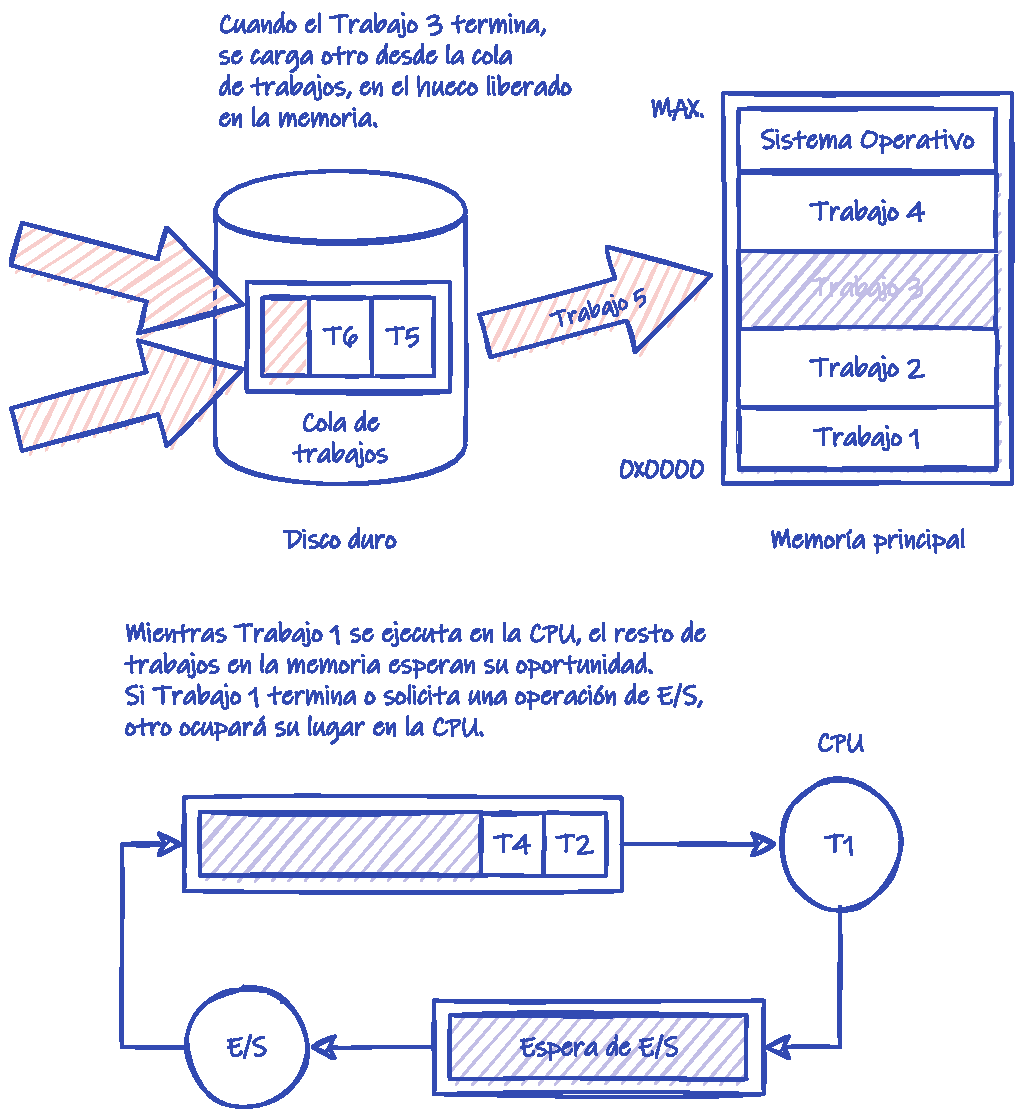
\includegraphics[width=0.8\textwidth]{media/C02_tipos_de_sistemas/sistemas_multiprogramados.pdf}
\caption{Gestión de trabajos en sistemas
multiprogramados.}\label{fig-sistemas-multiprogramados}
\end{figure}

En los \textbf{sistemas multiprogramados} la ejecución de los trabajos
funcionaba de la siguiente manera (véase la
\hyperref[fig-sistemas-multiprogramados]{Gestión de trabajos en sistemas
multiprogramados.}):

\begin{enumerate}
\def\labelenumi{\arabic{enumi}.}
\item
  En el disco magnético se almacenaba una cola donde se iban colocando
  todos los trabajos que tenían que ser ejecutados.
\item
  El sistema operativo cargaba varios trabajos en memoria del conjunto
  de trabajos en la cola en el disco magnético.
\item
  El sistema operativo cede la CPU a uno de los trabajos en memoria.
\item
  Cuando el trabajo en la CPU requería usar la E/S se lo pedía al
  sistema operativo. En lugar de mantener a la CPU ocupada inútilmente,
  el sistema operativo programaba la operación de E/S, pero escogía otro
  trabajo de entre los que estaban en memoria y lo ejecutaba en la CPU.

  Cuando la operación de E/S del anterior trabajo terminaba, el programa
  que ocupaba la CPU no era interrumpido, sino que debía esperar a una
  nueva oportunidad de ser escogido para ejecutarse en la CPU.
\item
  Cuando un programa en la CPU terminaba, sus recursos se liberaban,
  dejando memoria libre. Por lo tanto, el sistema operativo escogía un
  nuevo trabajo de la cola de trabajos en el disco magnético y lo
  cargaba en la memoria.
\end{enumerate}

Todo este proceso se repetía mientras hubiera trabajos que ejecutar en
la cola de trabajos en el disco.

Para operar de la forma descrita es necesario que el sistema operativo
realice tres tareas esenciales:

\begin{itemize}
\item
  La \textbf{planificación de trabajos}, cuya responsabilidad es
  seleccionar el siguiente trabajo que será cargado en la memoria
  principal para mantenerla llena.
\item
  La \textbf{planificación de la CPU}, cuya responsabilidad es elegir el
  siguiente trabajo que será ejecutado en la CPU, de entre los
  disponibles en la memoria principal.
\item
  La \textbf{gestión de la memoria}, cuya responsabilidad es repartir la
  memoria principal entre los trabajos alojados en la misma.
\end{itemize}

Un ejemplo de este tipo de sistemas operativos es el IBM OS/360, que fue
lanzado en 1966 para utilizarlo en los \emph{mainframes} IBM System/360
(véase el \hyperref[sect-historia-segunda-generaciuxf3n]{???}).

\subsection{Sistemas de tiempo
compartido}\label{_sistemas_de_tiempo_compartido}

{} Los sistemas multiprogramados ofrecían un uso más eficiente de la
CPU, pero no eran capaces de proporcionar interacción directa con los
usuarios. Los programadores seguían teniendo que entregar los trabajos
al operador y espera a que este les devolviera los resultados.

Los \textbf{sistemas de tiempo compartido} se desarrollaron tras
observar que al dar acceso a un grupo de usuarios se podía conseguir un
uso más eficiente del sistema, en comparación a cuando solo podía ser
utilizado por un usuario a la vez. Esto es debido a que, generalmente,
un usuario introduce información de forma continua para luego detenerse
durante largos periodos de tiempo, mientras que en un grupo de usuarios,
las pausas de uno de ellos se pueden llenar con la actividad de los
otros.

\begin{figure}
\centering
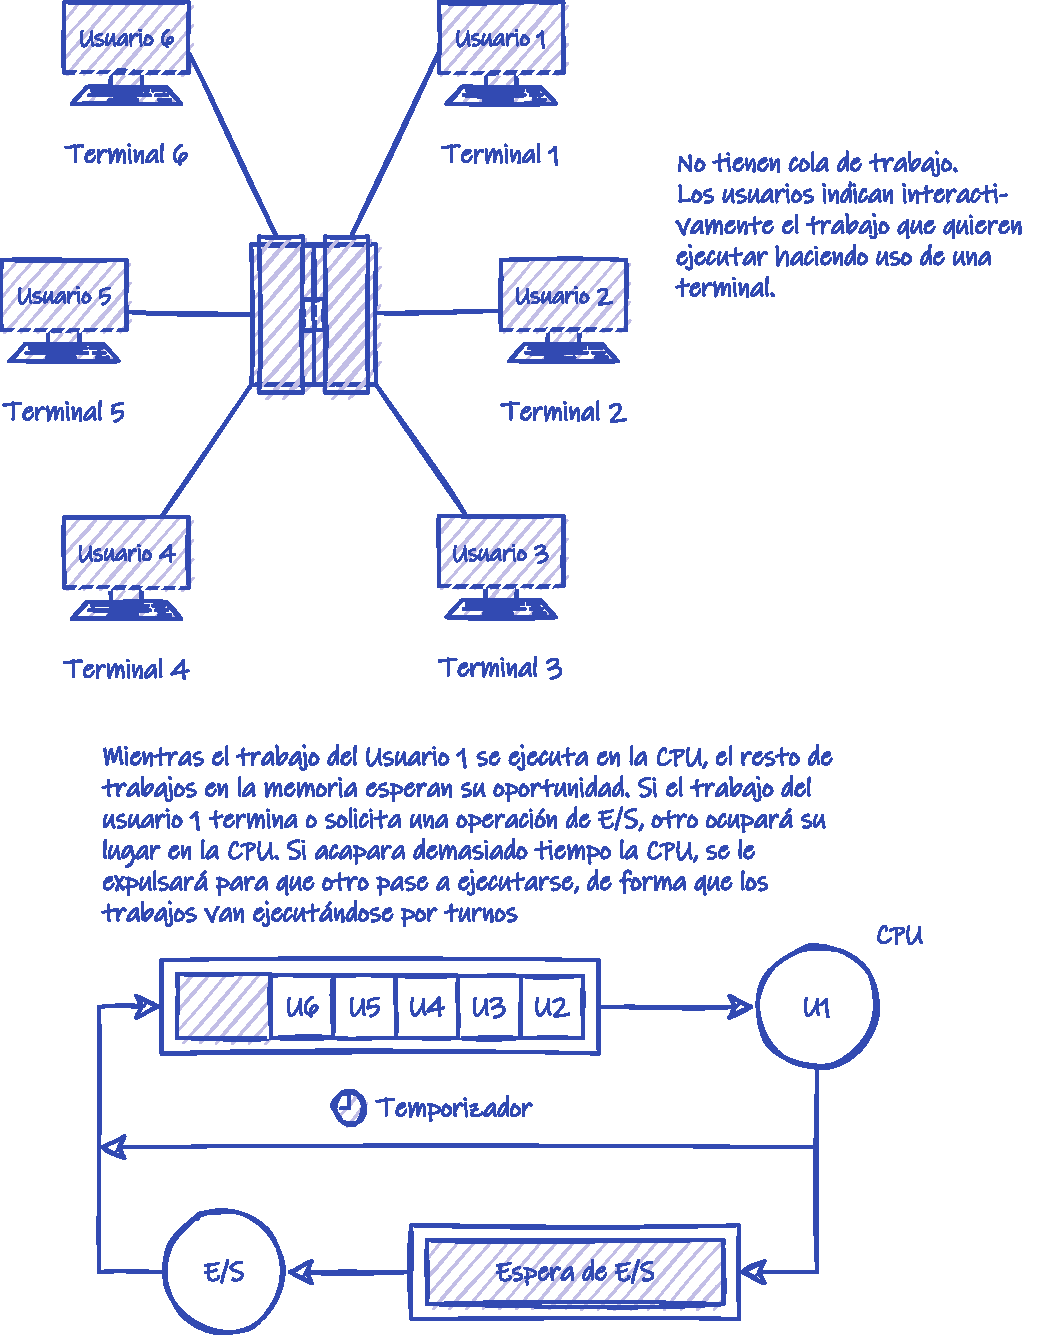
\includegraphics[width=0.8\textwidth]{media/C02_tipos_de_sistemas/sistemas_de_tiempo_compartido.pdf}
\caption{Gestión de trabajos en sistemas de tiempo
compartido.}\label{fig-sistemas-tiempo-compartido}
\end{figure}

Los \textbf{sistemas de tiempo compartido} se caracterizaban por:

\begin{itemize}
\item
  Tener \textbf{terminales}, es decir, hardware especializado en hacer
  de interfaz directa entre los usuarios y el sistema. A través de estas
  terminales los usuarios podían enviar comandos al sistema e
  interactuar con sus trabajos. Podía haber múltiples usuarios al mismo
  tiempo, pero cada uno solo podía tener un trabajo en ejecución a la
  vez.
\item
  Usar la \textbf{multiprogramación} para tener varios trabajos en la
  memoria principal al mismo tiempo e intercambiar el trabajo en la CPU
  cuando este solicitaba una operación de E/S, como ya se venía haciendo
  en los \textbf{sistemas multiprogramados} para hacer un uso más
  eficiente de la CPU.
\item
  Repartir el tiempo de CPU entre usuarios. El sistema operativo
  asignaba un tiempo de CPU a cada usuario ---denominado \textbf{ventana
  de tiempo} o \textbf{{}cuanto} de CPU---. Cuando este tiempo se
  agotaba, el sistema intercambiaba el trabajo en la CPU por el de otro
  usuario en el sistema. La ventana de tiempo era extremadamente
  pequeña, dando a cada usuario la impresión de que su trabajo nunca se
  detenía, como si dispusiera de la CPU en exclusiva.
\end{itemize}

Los sistemas que, como los de tiempo compartido, pueden ser utilizados
por varios usuarios simultáneamente se denominan sistemas
\textbf{{}multiusuario} {}.

En los primeros sistemas se usaban \textbf{{}terminales}
electromecánicos con un teclado y una impresora, como el
\href{https://en.wikipedia.org/wiki/Teletype_Model_33}{Teletype Model 3}
(1963). Posteriormente llegaron los terminales electrónicos, que usaban
un monitor en lugar de una impresora, como el
\href{https://es.wikipedia.org/wiki/IBM_3270}{IBM 3270}. En cualquier
caso solo disponían del hardware necesario para realizar la tarea de
conectar a los usuarios con el ordenador central.

Estos terminales no deben confundirse con las terminales por software
que traen algunos sistemas operativos modernos. Las terminales por
software o \emph{terminales virtuales} se programan para emular las
especificaciones de alguna versión de esas terminales físicas antiguas
que hemos comentado.

Los sistemas de tiempo compartido significaron un salto importante en
complejidad por diversas razones:

\begin{itemize}
\item
  Como varios trabajos están en la memoria principal al mismo tiempo, el
  sistema operativo requiere mecanismos de \textbf{gestión de la
  memoria} y \textbf{protección}.
\item
  Para tener un tiempo de respuesta razonable, los trabajos deben estar
  cargados en la memoria principal. Para que quepan más trabajos de los
  usuarios en la memoria, el sistema operativo debe utilizar técnicas de
  \textbf{memoria virtual} para ejecutar trabajos que no están
  completamente cargados en la memoria principal.
\item
  Como la CPU debe ser compartida entre todos los trabajos, el sistema
  operativo necesita mecanismos de \textbf{planificación de la CPU}.
\item
  Como varios trabajos pueden tener la necesidad de cooperar y que su
  ejecución siga cierto orden, el sistema operativo debe proporcionar
  mecanismos de \textbf{sincronización} y \textbf{comunicación}.
\item
  Como el sistema debe disponer de un \textbf{sistema de archivos} para
  repartir el espacio en disco y facilitar a los usuarios el acceso y
  gestión de sus datos, el sistema operativo necesita un componente de
  \textbf{gestión de discos}.
\end{itemize}

Las primeras versiones de UNIX ---lanzado por primera vez en 1970--- el
sistema operativo VMS ---desarrollado en 1978--- para los VAX de Digital
Equipment Corportation y el IBM OS/400 ---introducido en 1988---
utilizado en los minicomputadoras AS/400, son algunos ejemplos de
sistemas operativos de tiempo compartido (véase el
\hyperref[sect-historia-tercera-generaciuxf3n]{???}).

Estrictamente hablando, el término \textbf{sistemas de tiempo
compartido} hace referencia a estos \emph{mainframes} desarrollados a
partir de principios de la década de 1970. Así que no es común
utilizarlo con \emph{mainframes} modernos.

Los \emph{mainframes} modernos permiten a un mismo usuario ejecutar
varios trabajos al mismo tiempo, repartiendo el tiempo de CPU entre
todos los trabajo en el sistema y no solo entre los usuarios. Y lo mismo
ocurre en la mayor parte de los sistemas operativos de propósito general
actuales ---utilizados en ordenadores de escritorio, servidores,
portátiles y dispositivos móviles--- que con el tiempo han copiado
muchas características de los \textbf{sistemas de tiempo compartido}.
Por eso el término actual es \textbf{sistema multitarea}, que es mucho
más general.

La \textbf{{}multitarea} {} es un método para tener varios procesos en
memoria y ejecutarlos «al mismo tiempo». Generalmente requiere de
técnicas de multiprogramación, como las empleadas por los antiguos
\textbf{sistemas multiprogramados}, y de reparto del tiempo de CPU, como
ocurre en los antiguos \textbf{sistemas de tiempo compartido}. Por eso
se puede decir que ambos tipos de sistemas \emph{mainframe} eran
\textbf{sistemas multitarea}. Al igual que lo son los \emph{mainframes}
modernos y muchos sistemas operativos actuales de escritorio y de
dispositivos móviles.

\section{Sistemas de escritorio}\label{_sistemas_de_escritorio}

{} En la década de los 70 del siglo pasado también aparecieron las
primeras CPU en microprocesadores y con estas llegaron las
\textbf{microcomputadoras} o \textbf{microordenadores}. Las primeras
\textbf{{}microcomputadoras} no incluían teclado ni monitor y se
programaban usando interruptores y ledes ubicados en el frontal de la
unidad. Pero en torno a 1977 apareció la segunda generación de
\textbf{microcomputadoras}, que sí incluían estos periféricos de E/S,
por lo que eran más fáciles de usar que sus predecesoras. Entonces
comenzaron a recibir el nombre de \emph{ordenadores domésticos} y de su
mano llegaron los primeros \textbf{sistemas operativos de escritorio}.

\begin{figure}
\centering
\includegraphics[keepaspectratio]{media/C02_tipos_de_sistemas/ordenadores_domésticos_1977.jpg}
\caption{Los tres ordenadores que la revista Byte denominó como la
"Trinidad de 1977" de la computación doméstica: el
\href{https://es.wikipedia.org/wiki/Commodore_PET}{Commodore PET 2001},
el \href{https://es.wikipedia.org/wiki/Apple_II}{Apple II} y el
\href{https://es.wikipedia.org/wiki/TRS-80}{TRS-80 Model I} --- Fuente:
\href{https://commons.wikimedia.org/wiki/File:Trinity77.jpg}{Wikipedia}}\label{fig-ordenadores-domuxe9sticos-1977}
\end{figure}

Los \emph{mainframes} y las minicomputadoras de la época siguieron
siendo los ordenadores corporativos por excelencia, ya que eran mucho
más grandes y potentes, y también costosos.

El término en desuso \textbf{{}minicomputadora} o
\textbf{{}miniordenador} hace referencia a máquinas multiusuario de
rango medio, entre los \emph{mainframes} y los ordenadores domésticos.

Los primeros \textbf{sistemas operativos de escritorio} eran muy
básicos. Por ejemplo, en un sistema diseñado para ser utilizado por un
único usuario no tiene sentido implementar un sistema de archivos con
permisos. Así que, los primeros sistemas operativos de escritorio
carecían de esta característica que, sin embargo, ya existía en los
sistemas de tiempo compartido de la época. De la misma manera, carecían
de otros mecanismos de protección y no eran ni multiusuario ni
multitarea.

Pese a estas diferencias, los \textbf{sistemas operativos de escritorio}
se han beneficiado del desarrollo de los sistemas operativos para
\emph{mainframes}. Los sistemas de escritorio actuales son
\textbf{multiusuario} y \textbf{multitarea}; incluyen sistemas de
archivos con permisos, autenticación y mecanismos de protección de la
memoria ---como medidas para proteger los datos de los usuarios--- y han
incorporado muchas otras características de los sistemas operativos para
\emph{mainframe}.

Aunque con el tiempo los sistemas de escritorio han ido adquiriendo
características desarrolladas en los \emph{mainframes}, no debemos
olvidar que ambos tipos de sistemas se siguen diseñando con objetivos
diferentes. Mientras que en los \emph{mainframes} se persigue maximizar
la fiabilidad y utilización eficiente de los recursos, en los sistemas
de escritorio se maximiza la facilidad de uso y el tiempo de respuesta
al usuario, poniendo algo de atención al rendimiento.

Los \textbf{sistemas operativos de escritorio} modernos ya nos son «solo
de escritorio» ni se ejecutan únicamente en ordenadores domésticos. Se
utilizan en un altísimo porcentaje en servidores, superordenadores y
hasta en dispositivos móviles. Por eso, en la actualidad, el término
\textbf{sistema operativo de propósito general} {} es mucho más
adecuado.

El \textbf{tiempo de respuesta} al usuario se puede considerar como el
intervalo de tiempo entre un comando de un usuario ---por ejemplo un
clic--- y la respuesta del sistema a dicho comando. En ocasiones este
tiempo se minimiza a costa de un uso menos eficiente de los recursos del
sistema, por lo que no es un objetivo deseable para diseñar un
\emph{mainframe}. Para más información, véase el
\hyperref[_criterios_de_planificaciuxf3n]{???}.

Son muchos los ejemplos de sistemas operativos en esta categoría. Van
desde CP/M ---lanzado en 1977--- hasta los actuales GNU/Linux, Microsoft
Windows y Apple macOS, pasando por MS-DOS, IBM OS/2 y todas las
versiones anteriores de Microsoft Windows (véase el
\hyperref[sect-historia-cuarta-generaciuxf3n]{???}).

\section{Sistemas de mano}\label{_sistemas_de_mano}

{} {} Con el nombre genérico de \textbf{sistemas de mano} ---del inglés
\emph{handheld}--- hacemos referencia a las \emph{tablets},
\emph{smartphones}, lectores de libros electrónicos y otro sistemas
móviles y portátiles. Los desarrolladores de aplicaciones y sistemas de
mano deben enfrentarse a diversos desafíos, originados por el tamaño
limitado de los dispositivos y la alimentación mediante el uso de
baterías. Debido a esas limitaciones, muchos sistemas de mano tienen
poca cantidad de memoria, procesadores lentos ---en comparación con sus
equivalentes de escritorio--- y pantallas más pequeñas.

En el diseño del sistema operativo suele primar la facilidad de uso y
buscar un buen equilibrio entre rendimiento y tiempo de vida de la
batería.

\section{Sistemas multiprocesador}\label{_sistemas_multiprocesador}

{} Un \textbf{sistema multiprocesador} es aquel ordenador hay
procesadores interconectados que comparten el bus del sistema, el reloj
y, en ocasiones la memoria, y los periféricos.

Hace años esto solo se daba en sistemas con varias CPU, lo que era
relativamente común en servidores y sistemas de alto rendimiento para
trabajos técnicos o científicos. Sin embargo, en la actualidad cualquier
dispositivo digital u ordenador doméstico puede tener una CPU con
múltiples núcleos, lo que los convierte en sistemas multiprocesador.

Las principales ventajas de estos sistemas son:

\begin{itemize}
\item
  \textbf{Aumentan la cantidad de trabajo realizado}. A mayor número de
  procesadores, mayor cantidad de trabajo puede realizar el sistema. Sin
  embargo debemos de tener en cuenta que un sistema con \emph{N} CPU no
  es un sistema \emph{N} veces más rápido. Cuando varios procesadores
  cooperan para realizar una tarea, existe cierta pérdida de rendimiento
  debida a los mecanismos de sincronización requeridos para controlar el
  acceso a los recursos compartidos por los procesadores.
\item
  \textbf{Economía de escala}. Un sistema multiprocesador puede costar
  menos que múltiples sistemas monoprocesadores conectados para hacer un
  trabajo equivalente, porque comparten periféricos, almacenamiento,
  alimentación, etc.
\item
  \textbf{Alta disponibilidad}. Con el hardware adecuado el sistema
  puede ser tolerante al fallo de uno de los procesadores. En caso de
  fallo el sistema no se detendría, pero sí trabajaría más despacio.
\end{itemize}

En la actualidad existen dos tipos de sistemas multiprocesador:

\begin{figure}
\centering
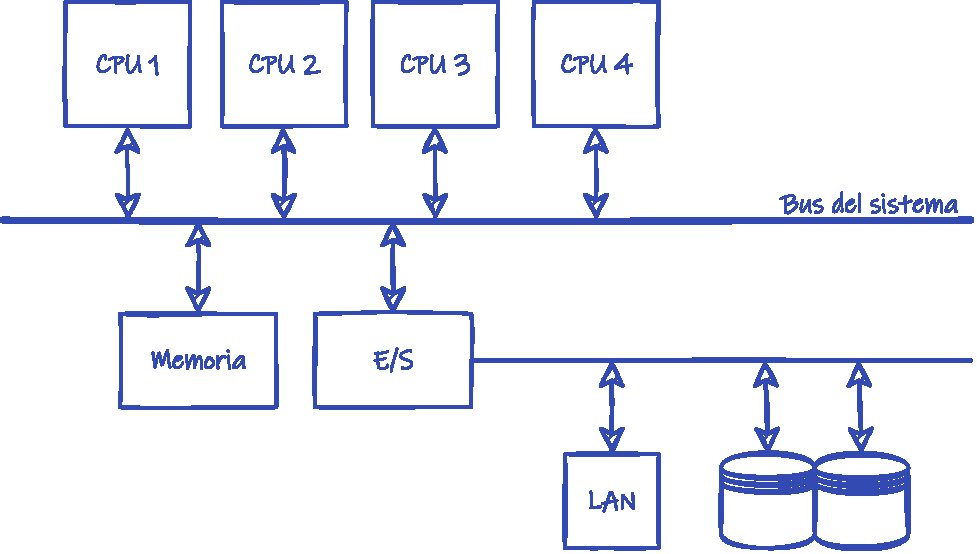
\includegraphics[width=0.8\textwidth]{media/C02_tipos_de_sistemas/multiprocesamiento_simétrico.pdf}
\caption{Arquitectura de un sistema de multiprocesamiento
simétrico.}\label{fig-smp}
\end{figure}

\begin{itemize}
\item
  En los \textbf{sistemas de multiprocesamiento simétrico}{}{} o
  \textbf{SMP} (\emph{Symmetric Multiprocessing}) todos los procesadores
  son iguales. Todos comparten los mismos recursos, pueden acceder a los
  mismos dispositivos (véase la \hyperref[fig-smp]{Arquitectura de un
  sistema de multiprocesamiento simétrico.}) y cada uno ejecuta una
  copia del núcleo del sistema operativo. El sistema operativo debe
  haber sido diseñado para saber repartir el trabajo entre los
  procesadores y compartir adecuadamente entre tareas y procesadores el
  resto de recursos del sistema. Casi todos los sistemas multiprocesador
  modernos son de este tipo.
\item
  En los \textbf{sistemas de multiprocesamiento asimétrico}{}{} o
  \textbf{AMP} (\emph{Asymmetric Multiprocessing}) hay un procesador
  principal y varios secundarios a quienes el principal planifica y
  entrega las tareas que deben ejecutar. En ocasiones los procesadores
  secundarios se distinguen del principal por haber sido diseñados para
  realizar algún tipo concreto de tareas de forma muy eficiente o por
  estar conectadas a hardware especial. Ejemplos de esto son las
  \href{https://es.wikipedia.org/wiki/Unidad_de_procesamiento_gr\%C3\%A1fico}{GPU},
  que no son sino procesadores diseñados específicamente para el
  procesamiento de gráficos, o las CPU de E/S conectadas a discos duros
  para gestionarlos de forma más eficiente.
\end{itemize}

Un ejemplo bastante ilustrativo es el de
\href{https://es.wikipedia.org/wiki/Cell_(microprocesador)}{Cell}, la
CPU de PlayStation 3. Tenía un núcleo principal de propósito general y 8
núcleos optimizados para ejecutar, de forma muy eficiente, operaciones
vectoriales. Con la ayuda del sistema operativo, los programas debían
envíar tareas matemáticamente intensivas a los procesadores secundarios,
si querían extraer el máximo provecho de la arquitectura.

Desarrollar para un sistema así es más complejo. Por lo que, aunque
sobre el papel esta arquitectura ofrecía gran rendimiento, aprovecharlo
era un verdadero reto para los desarrolladores.

\section{Sistemas distribuidos}\label{_sistemas_distribuidos}

{} En la actualidad es común el uso de redes para interconectar
ordenadores individuales ---por ejemplo Internet o la red de área local
de una oficina--- cada uno equipado con su procesador, su memoria, sus
dispositivos de almacenamiento, su fuente de alimentación, etc. En las
redes de ordenadores los procesadores de dichos ordenadores se comunican
con otros procesadores a través de líneas de comunicación, como: redes
Ethernet, líneas telefónicas o wifi. Estos sistemas son comúnmente
denominados \textbf{sistemas distribuidos}.

Sin entrar en detalles, los sistemas distribuidos pueden ser
clasificados en \textbf{sistemas cliente-servidor} y \textbf{sistemas de
redes entre iguales}.

\subsection{Sistemas cliente-servidor}\label{_sistemas_cliente_servidor}

En los \textbf{sistemas {}cliente-servidor} {} existen ordenadores que
actúan como \textbf{servidores} encargados de satisfacer las peticiones
generadas por otros ordenadores que actúan como \textbf{clientes}.

Este tipo de sistemas han sustituido, en un gran número de casos, a los
terminales conectados a \emph{mainframes}, debido a que los sistemas de
escritorio son cada vez más potentes y baratos. Concretamente:

\begin{itemize}
\item
  Los terminales han sido sustituidos por sistemas de escritorio que, al
  disponer de más recursos, son capaces de realizar muchas de las
  funcionalidades que anteriormente eran manejadas directamente por los
  \emph{mainframes}.
\item
  Al mismo tiempo estos \emph{mainframes} se han reemplazado por
  servidores, no muy diferentes a los sistemas de escritorios, pero
  preparados para atender las peticiones de sus clientes.
\end{itemize}

Ejemplos de este tipo de sistemas son los servidores de base de datos,
que responden a las consultas SQL de los clientes, o los servidores de
archivos, que proporcionan una interfaz de sistema de archivos con la
que los clientes pueden crear, leer, escribir y borrar archivos en el
servidor; de forma similar a como si estuvieran almacenados localmente
en el propio cliente.

\subsection{Sistemas de redes entre
iguales}\label{_sistemas_de_redes_entre_iguales}

En los \textbf{sistemas de redes entre iguales} {} {} o \textbf{{}P2P}
(\emph{peer-to-peer}) clientes y servidores no se distinguen los unos de
los otros. Todos los nodos del sistema son iguales y cada uno puede
actuar como cliente o servidor, dependiendo de cuándo piden o
proporcionan un servicio.

La ventaja fundamental de este tipo de sistemas es que en los sistemas
cliente-servidor el servidor puede ser el cuello de botella del
rendimiento, pero en los sistemas de redes entre iguales la carga se
distribuye entre todos los nodos de la red. Ejemplos de este tipo de
sistemas son las redes
\href{https://es.wikipedia.org/wiki/BitTorrent}{BitTorrent} y
\href{https://es.wikipedia.org/wiki/Bitcoin}{Bitcoin}.

Un servidor puede ser el cuello de botella no solo por su potencia sino
también por el ancho de banda de su conexión a la red. La potencia del
servidor es lo de menos cuando se intenta distribuir en Internet
archivos de gran tamaño ---por ejemplo imágenes de CD o DVD--- pues el
problema es que varias descargas simultáneas pueden consumir todo el
ancho de banda del servidor durante largos periodos de tiempo.

\subsection{Sistemas operativos para sistemas
distribuidos}\label{_sistemas_operativos_para_sistemas_distribuidos}

Desde el punto de vista de los sistemas operativos para sistemas
distribuidos es posible hacer la siguiente distinción:

\begin{itemize}
\item
  Los \textbf{sistemas operativos de red} {} ofrecen a las aplicaciones
  que corren sobre ellos servicios de acceso a redes de ordenadores. Por
  ejemplo, implementan algún mecanismo que permita a diferentes procesos
  en diferentes ordenadores enviar y recibir mensajes. Además suelen
  incorporar la opción de proporcionar algunos servicios de red, como la
  compartición de archivos y dispositivos con otros equipos de la misma
  red.

  Los ordenadores con sistemas operativos de red son autónomos.
  Simplemente es que gracias al sistema operativo de red, conocen la
  existencia de la red y saben usarla para comunicarse con otros
  ordenadores de la misma.

  Este tipo de sistemas operativos son los más utilizados en los tipos
  de sistemas distribuidos comentados anteriormente. En la actualidad,
  la inmensa mayoría de sistemas de escritorio y dispositivos de mano
  utilizan sistemas operativos de red.
\item
  Los \textbf{sistemas operativos distribuidos} {} crean en el usuario
  la ilusión de que está en un único ordenador, aunque en realidad el
  sistema operativo controla todos los ordenadores de la red, dando al
  usuario acceso transparente a los recursos en todos los equipos de la
  misma.

  Con este tipo de sistemas operativos el usuario no sabe en qué
  ordenador se ejecutan sus procesos, donde se almacenan sus archivos,
  ni qué equipo tiene conectado los distintos periféricos a los que
  tiene acceso.
\end{itemize}

Un ejemplo de sistema operativo distribuido es
\href{https://en.wikipedia.org/wiki/Amoeba_(operating_system)}{Amoeba},
un sistema operativo distribuido de investigación escrito por Andrew S.
Tanenbaum en Vrije Universiteit. Para más información, véase el
\href{http://www.cs.vu.nl/pub/amoeba/}{sitio web de Amoeba}.

\section{Sistemas en clúster}\label{_sistemas_en_cluxfaster}

{} Como los sistemas distribuidos, los \textbf{sistemas en clúster}
interconectar ordenadores individuales. Sin embargo, generalmente se
acepta que los \textbf{sistemas en clúster} comparten el almacenamiento
y estén conectados por medio de una red local, condiciones que no tienen
por qué darse en los sistemas distribuidos.

Los \textbf{sistemas en clúster} se utilizan para:

\begin{itemize}
\item
  \textbf{Obtener servicios con alta disponibilidad}. Para ello un nodo
  del clúster puede estar ejecutando un servicio mientras otro nodo lo
  monitoriza. En caso de fallo en el nodo que da el servicio, el que lo
  monitoriza lo sustituye.

  Si es necesario proporcionar varios servicios, el mecanismo anterior
  se puede extender repartiendo los servicios entre dos o más nodos y
  haciendo que se monitoricen entre ellos.
\item
  \textbf{Computación de alto rendimiento} o \textbf{HPC}. En este caso
  todos los nodos se utilizan para dar un mismo servicio. Un nodo
  especial, denominado balanceador de carga, tiene la responsabilidad de
  repartir el trabajo entre los nodos.

  Este tipo de \textbf{sistemas en clúster} se utiliza para realizar
  trabajos de cálculo muy pesados, como simulaciones ---por ejemplo
  simulación meteorológica, nuclear o de gestión hospitalaria--- o
  romper sistemas de cifrado.
\end{itemize}

También es muy utilizado en servidores de Internet ---como servidores
web, correo electrónico o de mensajería instantánea--- o servidores de
base de datos que deben dar servicio a una gran cantidad de clientes
simultáneamente. En estos casos el balanceador de carga realiza su
trabajo repartiendo las conexiones de los usuarios entre los servidores
del clúster.

\section{Sistemas de tiempo real}\label{_sistemas_de_tiempo_real}

{} Los \textbf{sistemas de {}tiempo real} se utilizan cuando existen
requerimientos estrictos de tiempo en la ejecución de ciertas tareas o
en el procesamiento de flujos de datos.

En general se usan frecuentemente en dispositivos de control donde,
dentro de unos márgenes estrictos de tiempo, se deben tomar datos de uno
o varios sensores, para analizarlos posteriormente y realizar, en
consecuencia, alguna acción con algún mecanismo de control. Por ejemplo,
se suelen utilizar en sistemas de control industrial, domótica,
armamento, automoción ---en la inyección electrónica de combustible,
sistemas de frenado y de control de tracción--- o en dispositivos
médicos.

Los \textbf{sistemas de tiempo real} están muy relacionados con los
\textbf{sistemas empotrados}{}. Estos últimos:

\begin{itemize}
\item
  Se diseñan para realizar tareas muy específicas. No son sistemas de
  propósito general sino de propósito específico.
\item
  Sus sistemas operativos tienen características muy limitadas y no
  tienen que tener necesariamente una interfaz de usuario.
\item
  Estos sistemas están tanto en el motor de los automóviles y los robots
  que los fabrican, como en reproductores de DVD, microondas o
  dispositivos de red.
\end{itemize}

Los \textbf{sistemas de tiempo real} pueden ser clasificados en
\textbf{sistemas de tiempo real estricto} y \textbf{sistemas de tiempo
real flexible}:

\begin{itemize}
\item
  Los \textbf{sistemas de tiempo real estricto} {}{} o \textbf{{}hard
  real-time} garantizan que las tareas serán realizadas dentro de unos
  márgenes estrictos de tiempo.

  Para ello, todas las situaciones imprevistas que puedan ocasionar
  retrasos en el funcionamiento del sistema operativo deben estar
  perfectamente delimitadas en tiempo. Por lo tanto, suelen carecer de
  memoria virtual y de otras abstracciones que aíslen al desarrollador
  del funcionamiento real del hardware, ya que introducen
  impredecibilidad.

  Los sistemas de tiempo real estricto no son compatibles con los
  sistemas de tiempo compartido.
\item
  Los \textbf{sistemas de tiempo real flexible} {} {} o \textbf{{}soft
  real-time} son útiles cuando en un sistema operativo convencional hay
  tareas que tienen mayor importancia que el resto, por lo que deben ser
  realizadas con mayor prioridad.

  El tiempo real flexible no sirve cuando se tienen tareas con
  limitaciones precisas de tiempo, porque no hay manera de garantizar
  que dichas restricciones se van a cumplir. Sin embargo sí es útil para
  tareas relacionadas con la multimedia, la realidad virtual, los
  videojuegos, etc. y es compatible con la memoria virtual y otras
  características presentes en los sistemas de escritorio. Por eso la
  mayor parte de los sistemas de escritorio actuales soportan tareas de
  tiempo real flexible.
\end{itemize}
